\subsection{Hyperparameter Choice Justification} \label{sec:A2}
Our hyperparameters are $L$ and $\theta$. Recall that $L$ denotes the number of trading days over which we hold the positions in the beta-neutral strategy, while $\theta$ represents the upper bound on each side (long and short) for the amount of clusters we select for the trading strategy. The specific choice of hyperparameters we made for the results presented in the paper were:
\begin{align*}
L &= 4
\\
\theta &= \integer{0.5k}
\end{align*}
where $k$ represents the number of clusters (26 for KMeans clustering, and 20 for LLM clustering). This choice is not arbitrary nor opportunistic. Instead, it results from the maximization of the Sharpe Ratio of the portfolio in the train and validation samples for both KMeans and LLM clustering. This choice procedure is completely based on \textit{in-sample} criteria and it prevents lookahead bias. The justification for such choices is made below.

\subsubsection{KMeans Clustering}

In \cref{fig:KMeans_hyperparameter_justification_L} we can see that a choice of $L=4$ in the training and validation splits generates the most stable Sharpe Ratio. Namely, In the train set (\cref{fig:K_hyp_1}), it makes more sense to choose low values of $L$ (less than 4) to maximize the $SR$. However, in the validation set (\cref{fig:K_hyp_2}), it makes more sense to choose higher values of $L$. The choice of $L=4$ represents a balanced compromise, providing a stable Sharpe Ratio profile across both splits, ensuring consistent in-sample performance.
%The choice of $L=4$ stands as a middle ground between this contradiction, generating a stable choice and a stable profile of earnings in sample.

\setcounter{figure}{0}
%----------------------------------------------------
\inserthere{fig:KMeans_hyperparameter_justification_L}
\begin{figure}[H]
  \caption{Sharpe Ratios in the train and validation splits as a function of $L$ (KMeans)}
  \centering
  
  \begin{subfigure}[b]{0.46\textwidth}
    \centering
    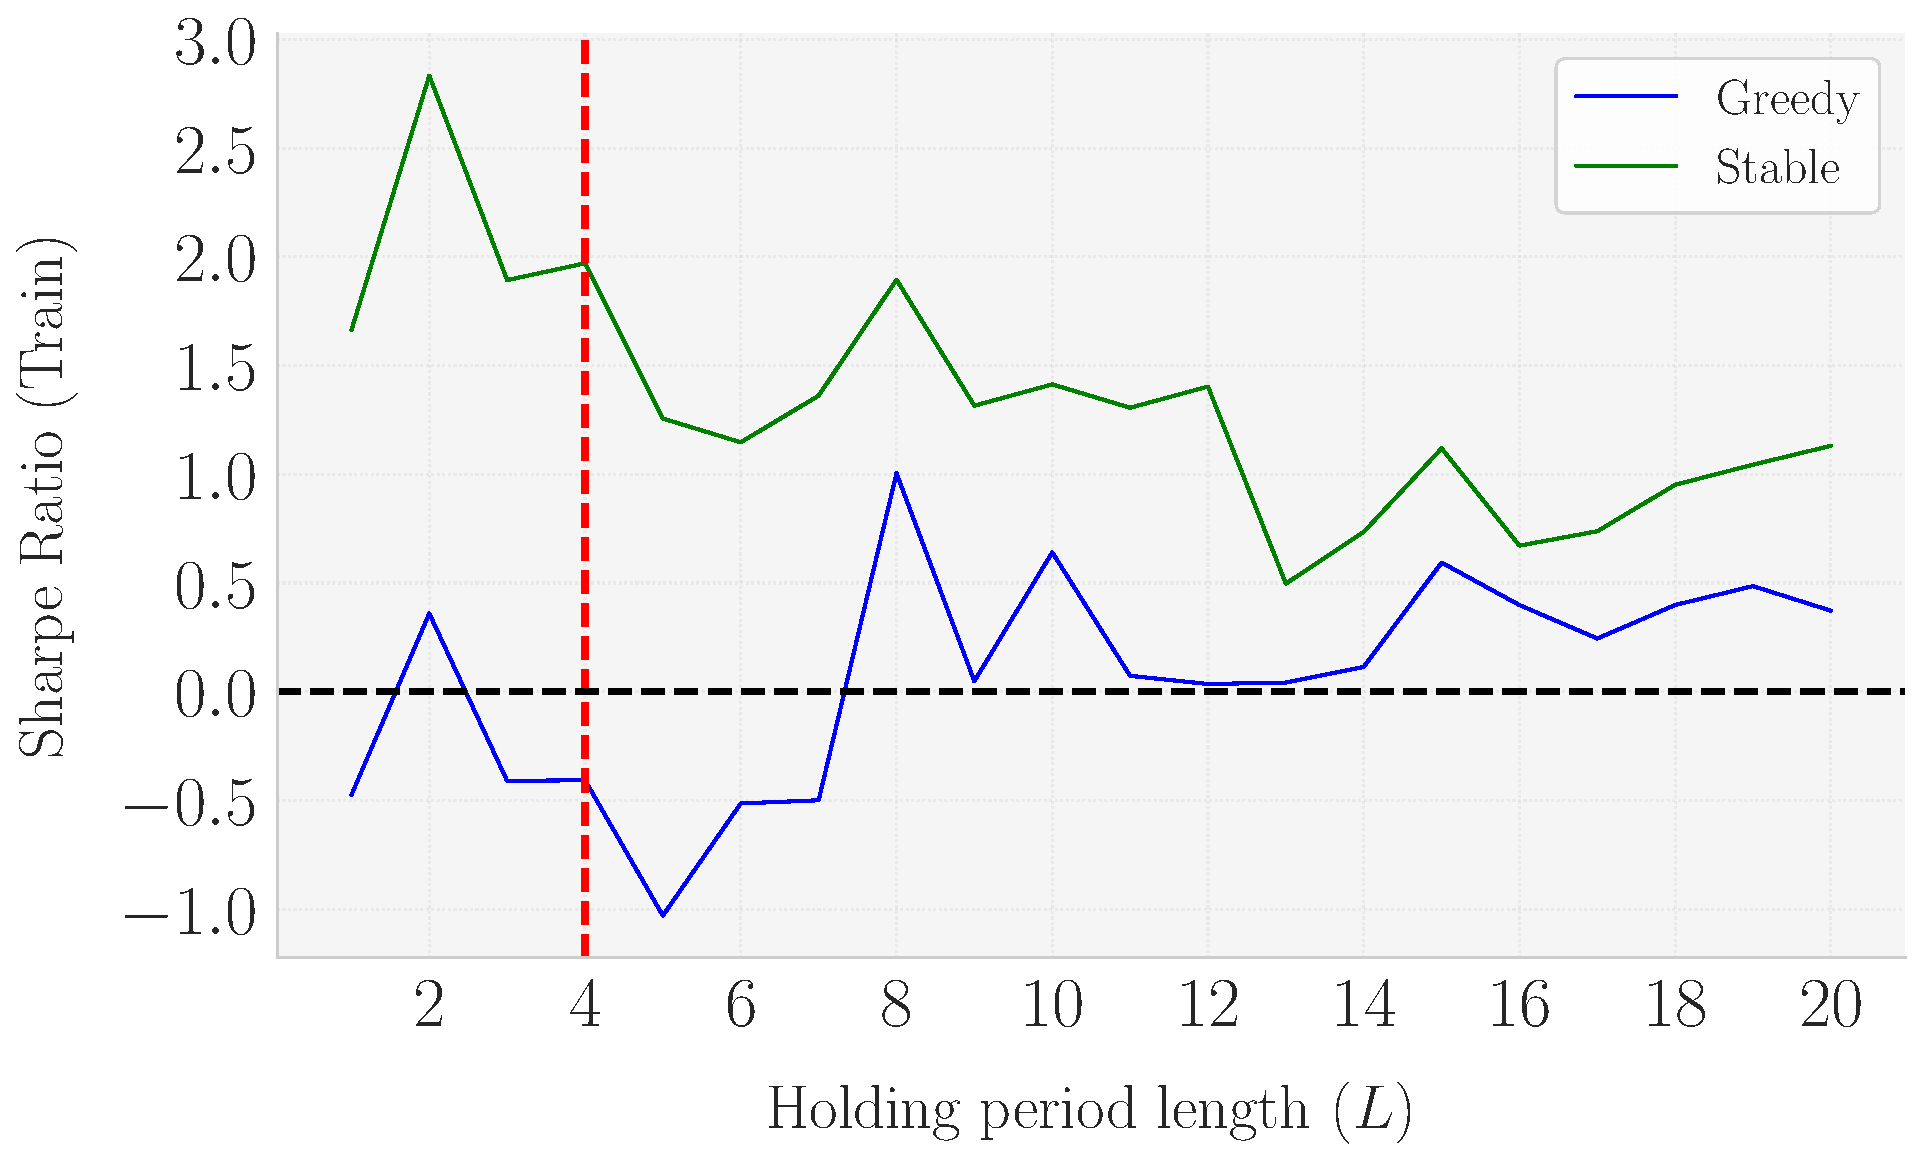
\includegraphics[width=\textwidth]{fig_A1a_KMeans_SR_Train_vs_L.pdf}
    \caption{Plot of $SR^{\mathcal P^{tr}}(L)$ over a grid of $L$}
    \label{fig:K_hyp_1}
  \end{subfigure}
  \hspace{0.05\textwidth} % Add horizontal space between the subfigures
  \begin{subfigure}[b]{0.46\textwidth}
    \centering
    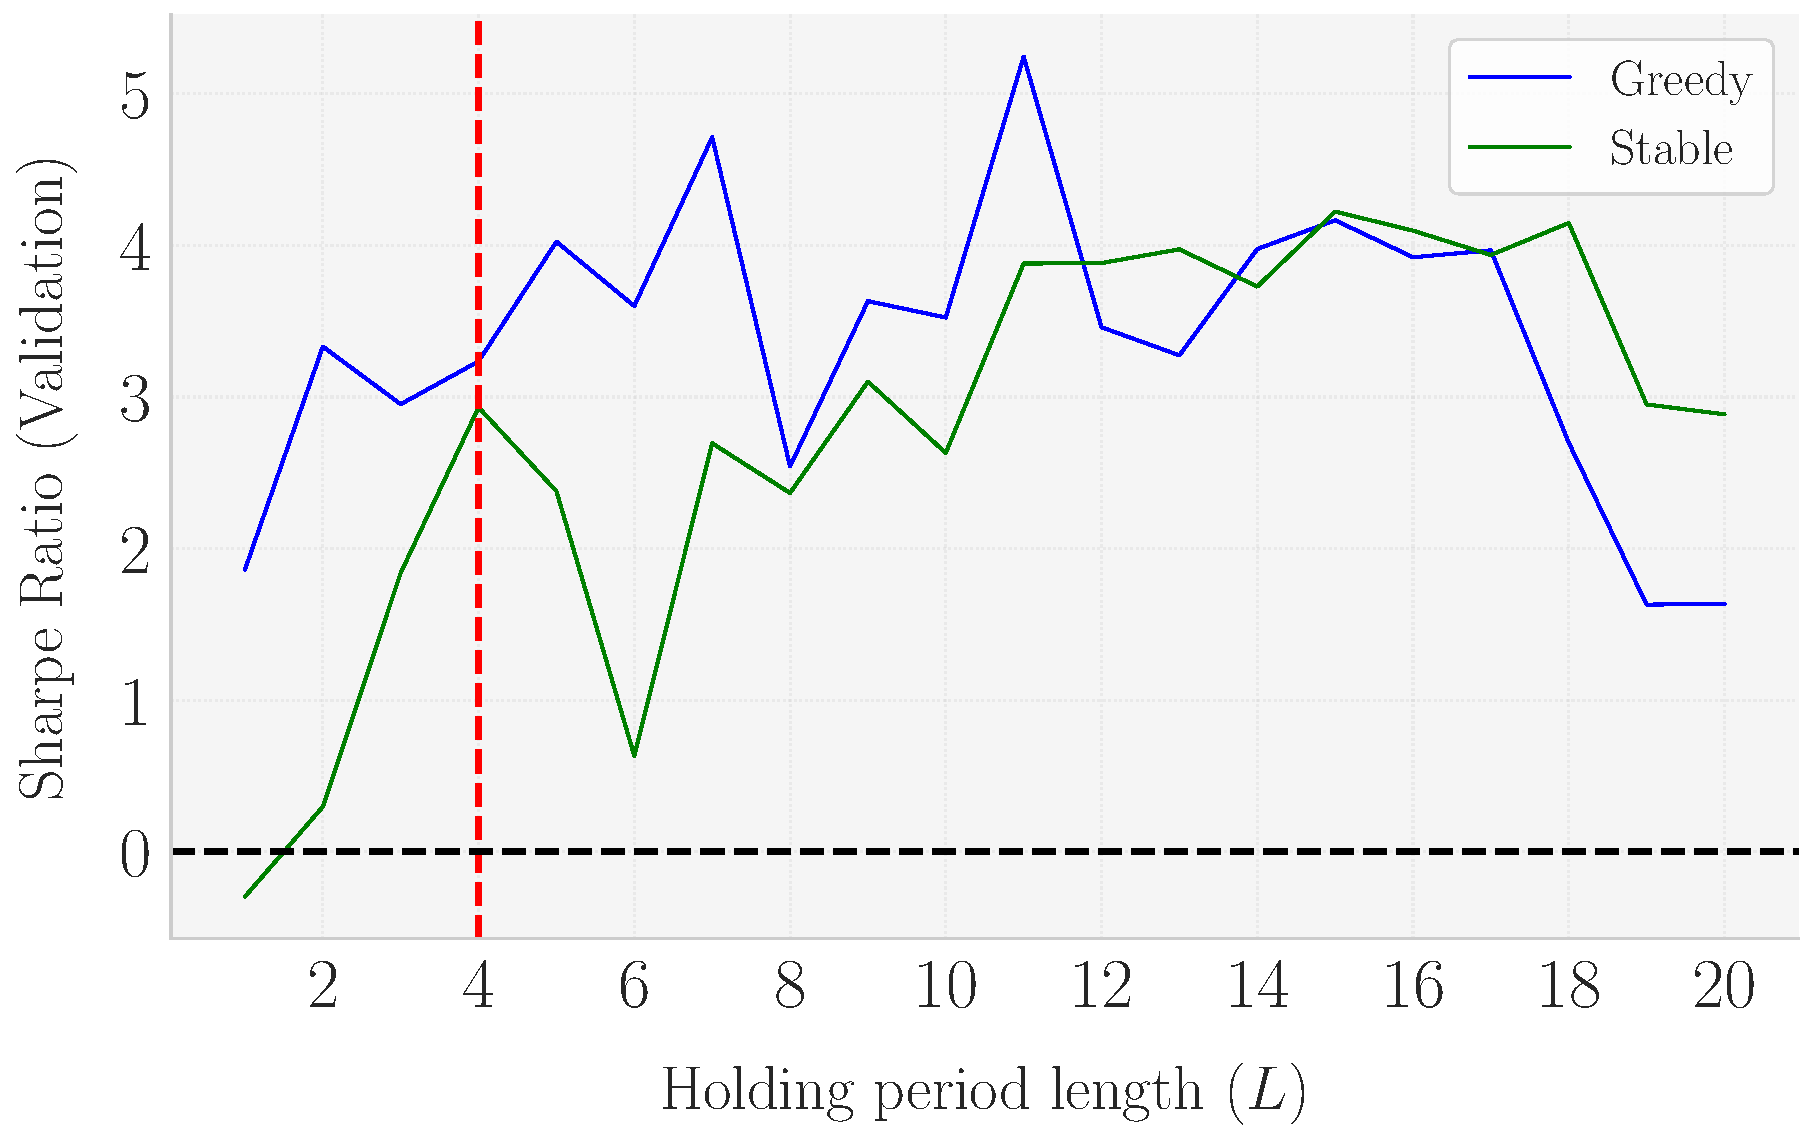
\includegraphics[width=\textwidth]{fig_A1b_KMeans_SR_Validation_vs_L.pdf}
    \caption{Plot of $SR^{\mathcal P^{val}}(L)$ over a grid of $L$}
    \label{fig:K_hyp_2}
  \end{subfigure}  
  \mx
  \subcaption*{\textit{Note: This figure shows the Sharpe Ratios ($SR$) as a function of the holding period length ($L$) for the KMeans clustering method in the training (Panel a) and validation (Panel b) splits. In Panel (a), the Sharpe Ratios in the training set indicate that lower values of $L$ (less than 4) maximize performance. Conversely, in Panel (b), the validation set shows higher Sharpe Ratios for longer holding periods. The choice of $L=4$ represents a balanced compromise, providing a stable Sharpe Ratio profile across both splits, ensuring consistent in-sample performance without introducing lookahead bias.}}
  \label{fig:KMeans_hyperparameter_justification_L}
\end{figure}
%----------------------------------------------------

On the other hand, the choice of $\theta=\integer{0.5\cd 26}=13$ is a choice that pursues stability in the Sharpe Ratio of the train and validation portfolios. As we can see from \cref{fig:KMeans_hyperparameter_justification_theta}, the Sharpe Ratios tend to converge to the highest and most stable value when we choose the highest possible value of $\theta$. 

 %----------------------------------------------------
\inserthere{fig:KMeans_hyperparameter_justification_theta}
\begin{figure}[H]
  \caption{Sharpe Ratios in the train and validation splits as a function of $\theta$ (KMeans)}
  \centering
    \begin{subfigure}[b]{0.46\textwidth}
    \centering
    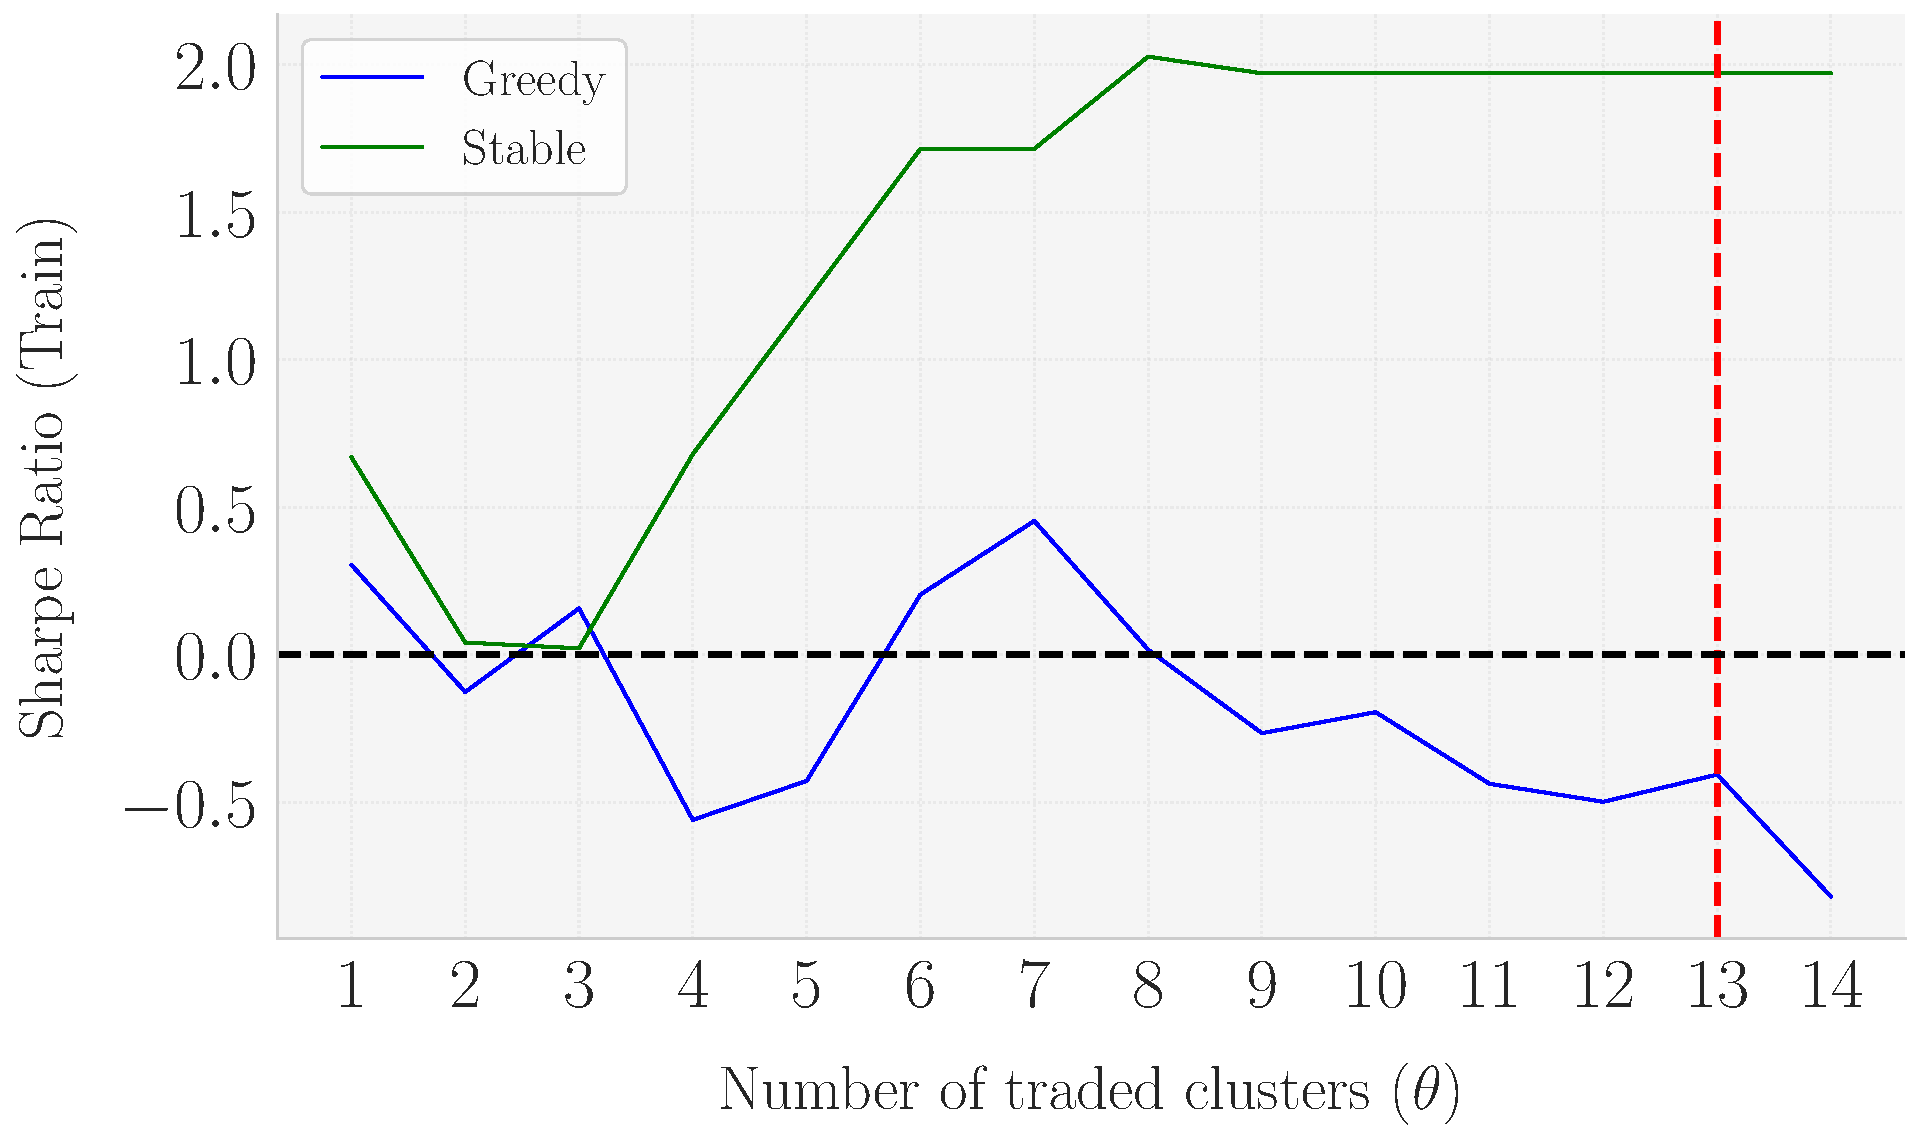
\includegraphics[width=\textwidth]{fig_A2a_KMeans_SR_Train_vs_theta.pdf}
    \caption{Plot of $SR^{\mathcal P^{tr}}(\theta)$ over a grid of $\theta$}
    \label{fig:K_hyp_3}
  \end{subfigure}
  \hspace{0.05\textwidth} % Add horizontal space between the subfigures
  \begin{subfigure}[b]{0.46\textwidth}
    \centering
    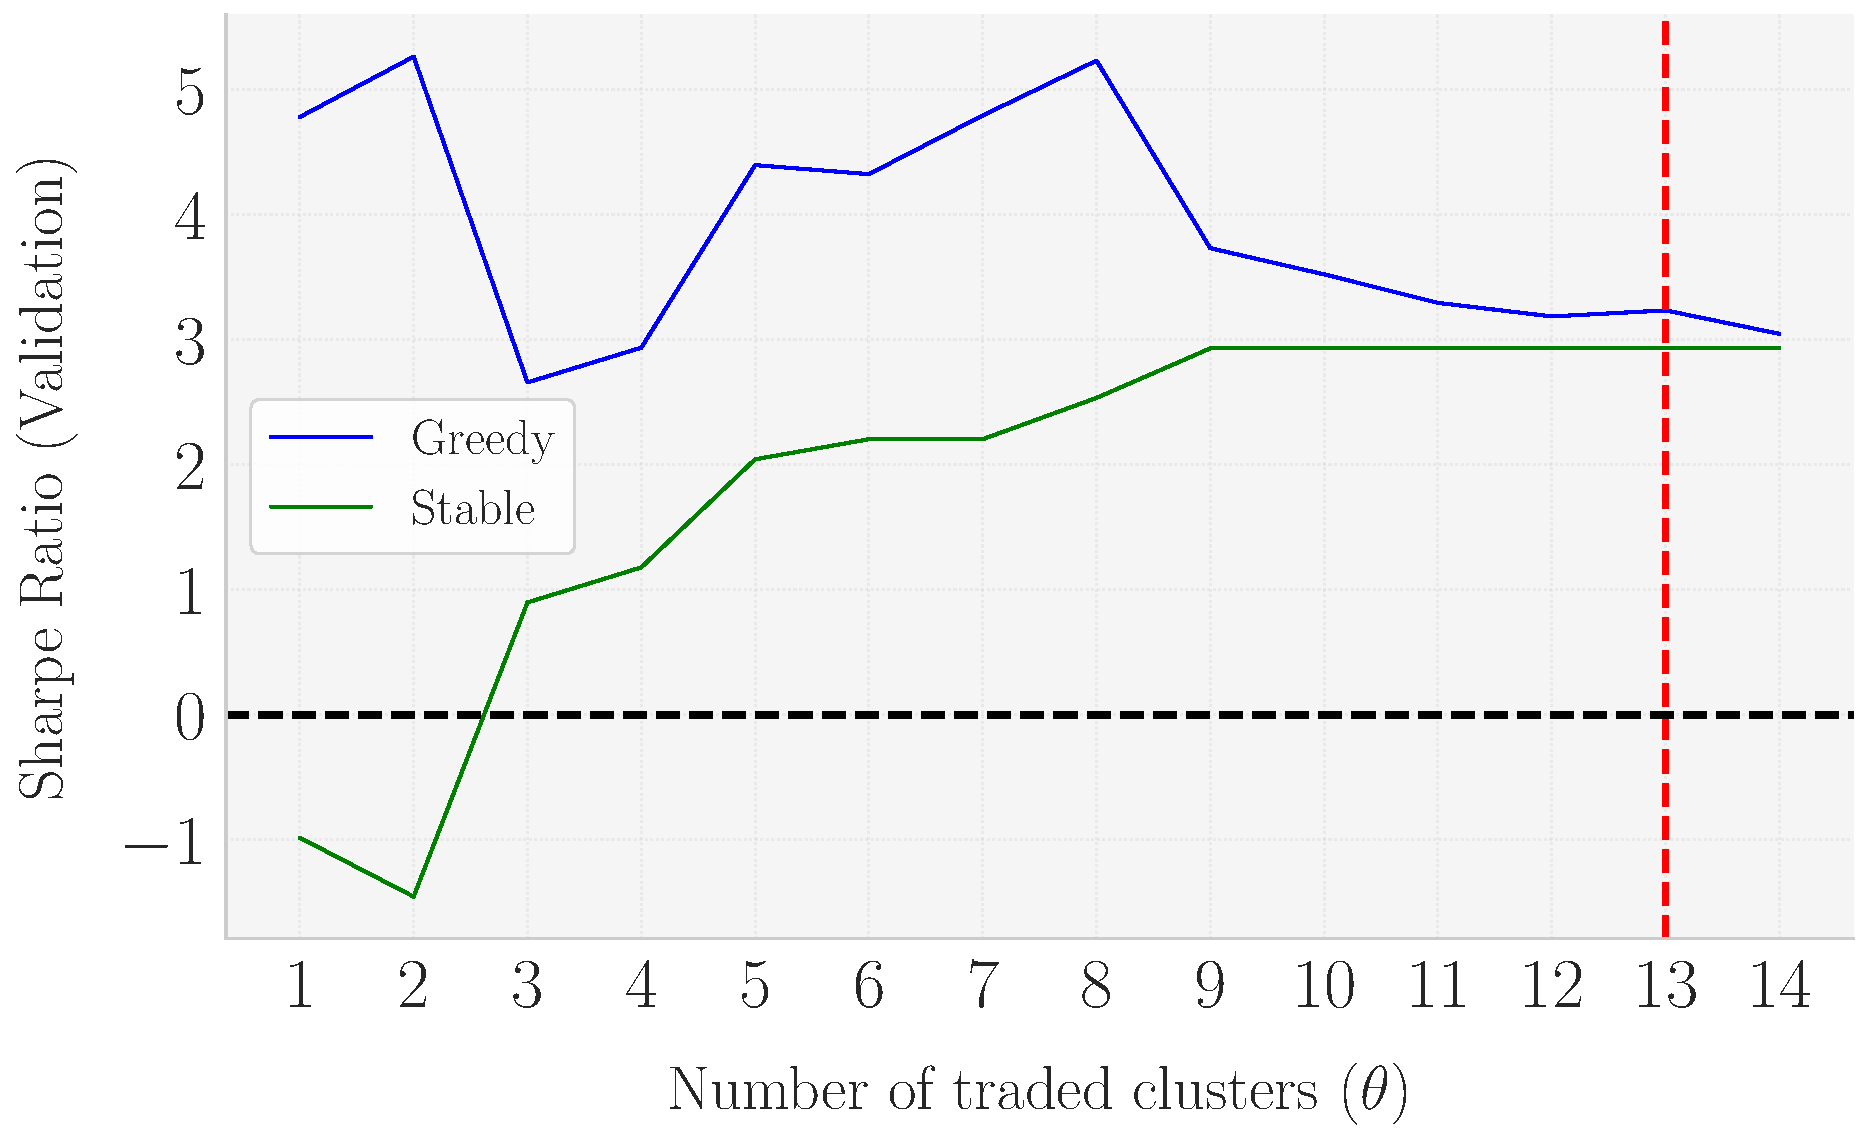
\includegraphics[width=\textwidth]{fig_A2b_KMeans_SR_Validation_vs_theta.pdf}
    \caption{Plot of $SR^{\mathcal P^{val}}(\theta)$ over a grid of $\theta$}
    \label{fig:K_hyp_4}
  \end{subfigure}
  \mx
\subcaption*{\textit{Note: This figure illustrates the Sharpe Ratios ($SR$) as a function of $\theta$, the upper bound on the number of traded clusters, for the KMeans clustering method in the training (Panel a) and validation (Panel b) splits. In Panel (a), the Sharpe Ratios in the training set show a trend of increasing stability and maximizing performance as $\theta$ approaches its upper limit. Similarly, Panel (b) displays a consistent pattern in the validation set, where higher values of $\theta$ lead to convergence at the highest and most stable Sharpe Ratios. The choice of $\theta = 13$ (i.e: $\integer{0.5 \cdot 26}$) reflects this observed stability and optimization, providing a balanced and robust selection for the portfolio strategy.}}
  \label{fig:KMeans_hyperparameter_justification_theta}
\end{figure}
%----------------------------------------------------


\subsubsection{LLM Clustering}
Following a similar logic as below, the choice of $L=4$ sets a consensus between the maximization of $SR^{\mathcal P^{tr}}$ and $SR^{\mathcal P^{val}}$. That is, maximizing $SR^{\mathcal P^{tr}}$ requires lower holding period lengths (the maximizer is $L=4$), while maximizing $SR^{\mathcal P^{val}}$ requires increasing the window length. Among this contradiction, from \cref{fig:LLM_hyperparameter_justification_L} it follows that $L=4$ stands as a perfect choice to balance the maximization requirements in both samples, generating a stable choice for the holding period window length.

%----------------------------------------------------
\inserthere{fig:LLM_hyperparameter_justification_L}
\begin{figure}[H]
  \caption{Sharpe Ratios in the train and validation splits as a function of hyperparameters (LLM)}
  \centering
  
  \begin{subfigure}[b]{0.46\textwidth}
    \centering
    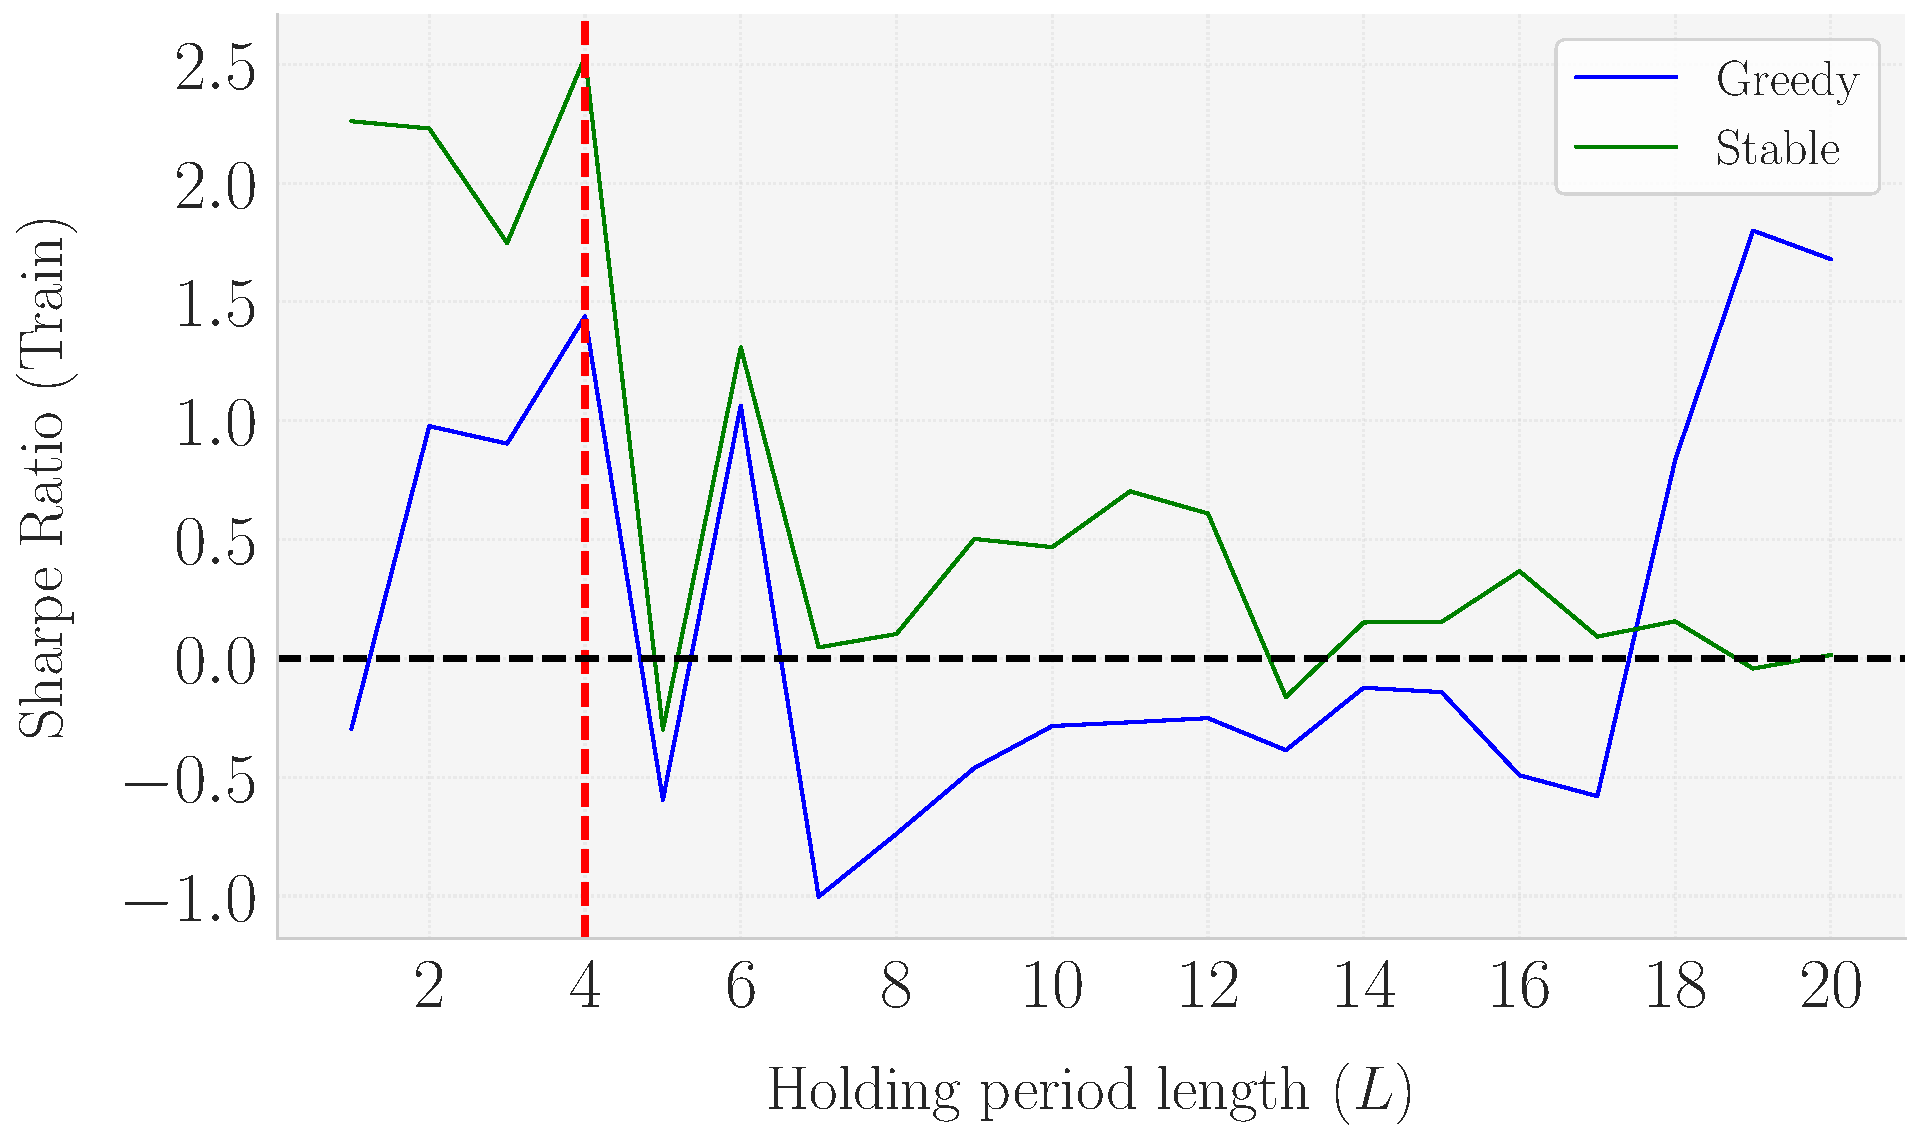
\includegraphics[width=\textwidth]{fig_A3a_LLAMA_SR_Train_vs_L.pdf}
    \caption{Plot of $SR^{\mathcal P^{tr}}(L)$ over a grid of $L$}
    \label{fig:LLM_hyp_1}
    
  \end{subfigure}
  \hspace{0.05\textwidth} % Add horizontal space between the subfigures
  \begin{subfigure}[b]{0.46\textwidth}
    \centering
    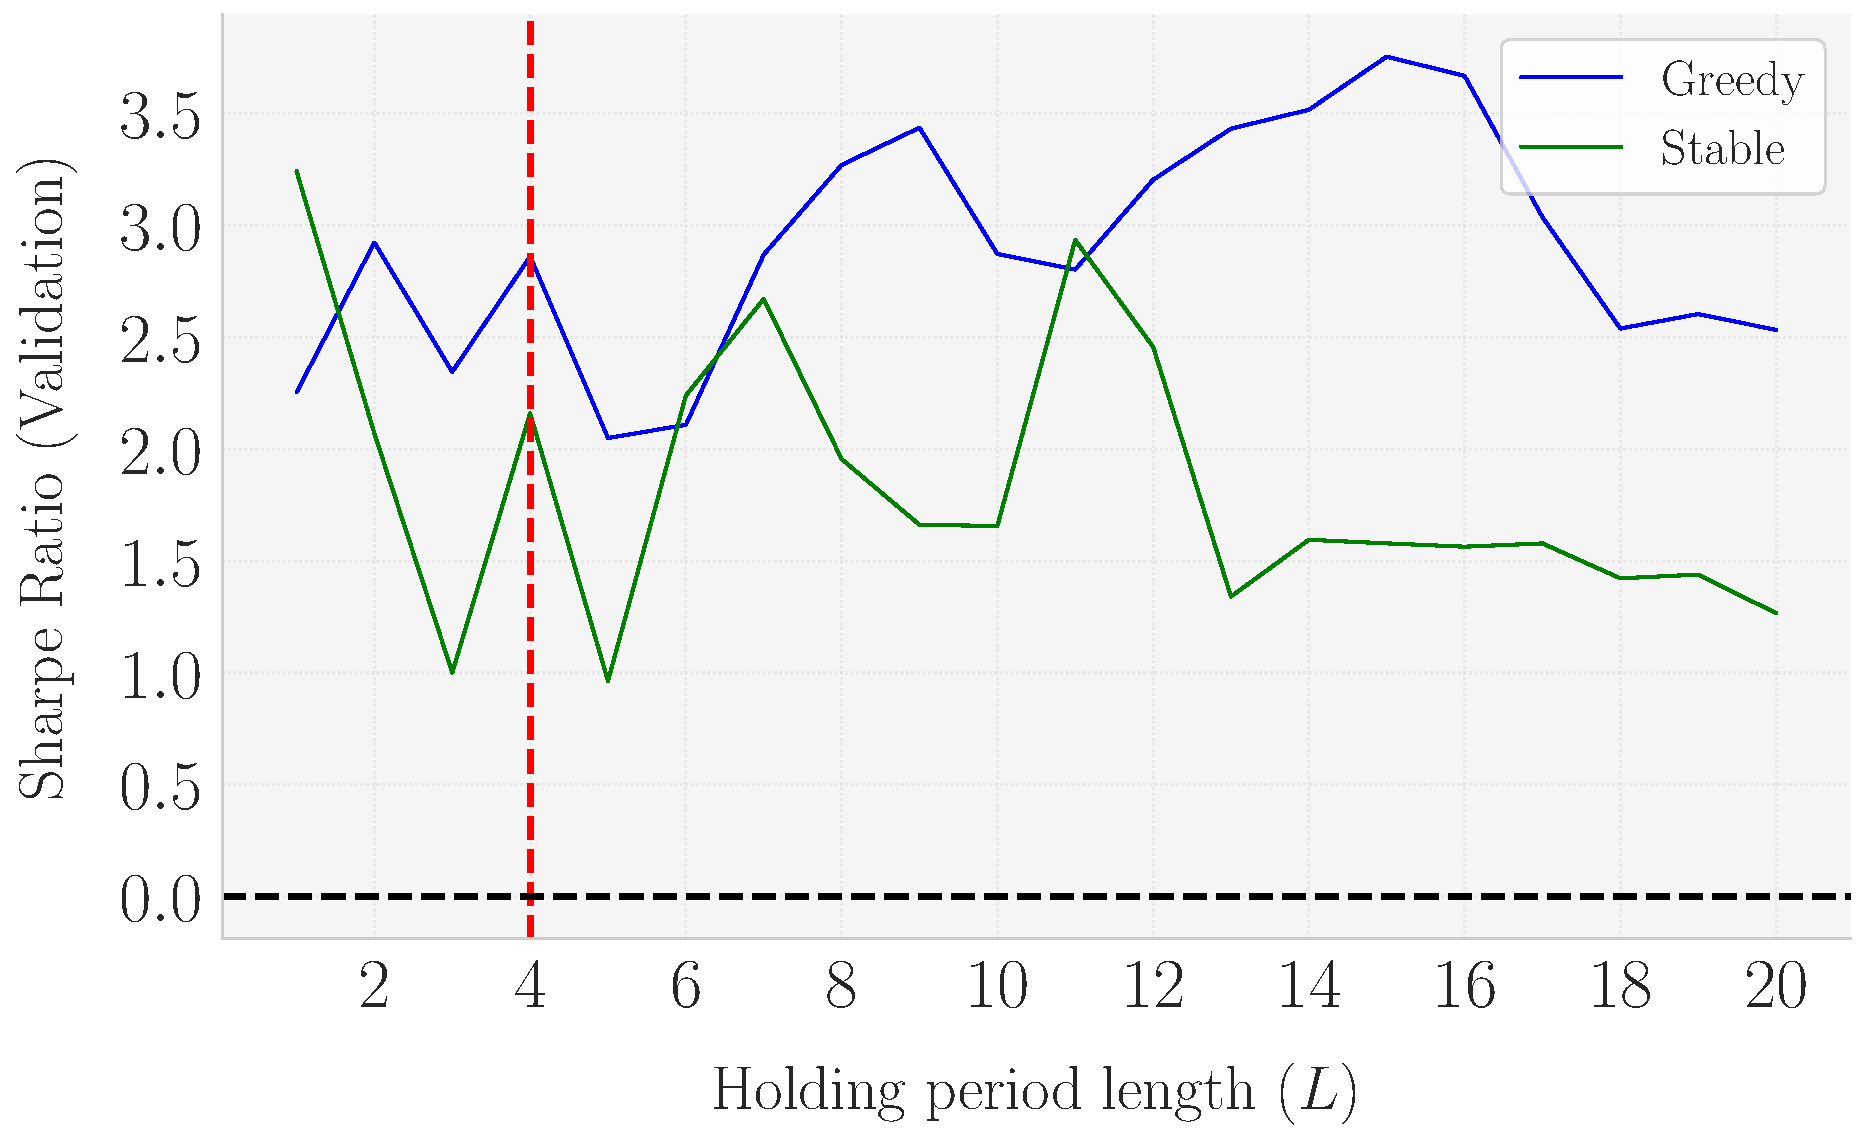
\includegraphics[width=\textwidth]{fig_A3b_LLAMA_SR_Validation_vs_L.pdf}
    \caption{Plot of $SR^{\mathcal P^{val}}(L)$ over a grid of $L$}
    \label{fig:LLM_hyp_2}
  \end{subfigure}
  \mx 
  \subcaption*{\textit{Note: This figure shows the Sharpe Ratios ($SR$) as a function of the holding period length ($L$) for the LLM clustering method, across the training (Panel a) and validation (Panel b) splits. In Panel (a), the Sharpe Ratios in the training set reach their maximum at $L=4$, suggesting shorter holding periods are more effective for maximizing performance. Conversely, Panel (b) illustrates that longer holding periods yield higher Sharpe Ratios in the validation set. The choice of $L=4$ serves as a compromise, balancing the trade-off between maximizing $SR$ in both splits and providing a stable and consistent holding period length for the strategy.}}
  \label{fig:LLM_hyperparameter_justification_L}
\end{figure}
%----------------------------------------------------

Finally, the same conclusion as in KMeans applies here. By selecting $\theta=\integer{0.5\cd 20}=10$, we get a stable Sharpe Ratio. Even though we observe that $SR^{\mathcal P^{tr}}(L)$ falls momentarily at $\theta=10$ for the Greedy algorithm, it still constitutes a good choice. Conversely, at $\theta=10$ the greedy algorithm sees a jump in $SR^{\mathcal P^{val}}(L)$ (see \cref{fig:LLM_hyperparameter_justification_theta}). All in all, we can easily conclude that $\theta=\integer{0.5k}$ arises as a good hyperpamrameter choice also for LLM clustering.
%----------------------------------------------------
\inserthere{fig:LLM_hyperparameter_justification_theta}
\begin{figure}[H]
\caption{Sharpe Ratios in the train and validation splits as a function of $\theta$ (LLM)}
  \centering

    \begin{subfigure}[b]{0.46\textwidth}
    \centering
    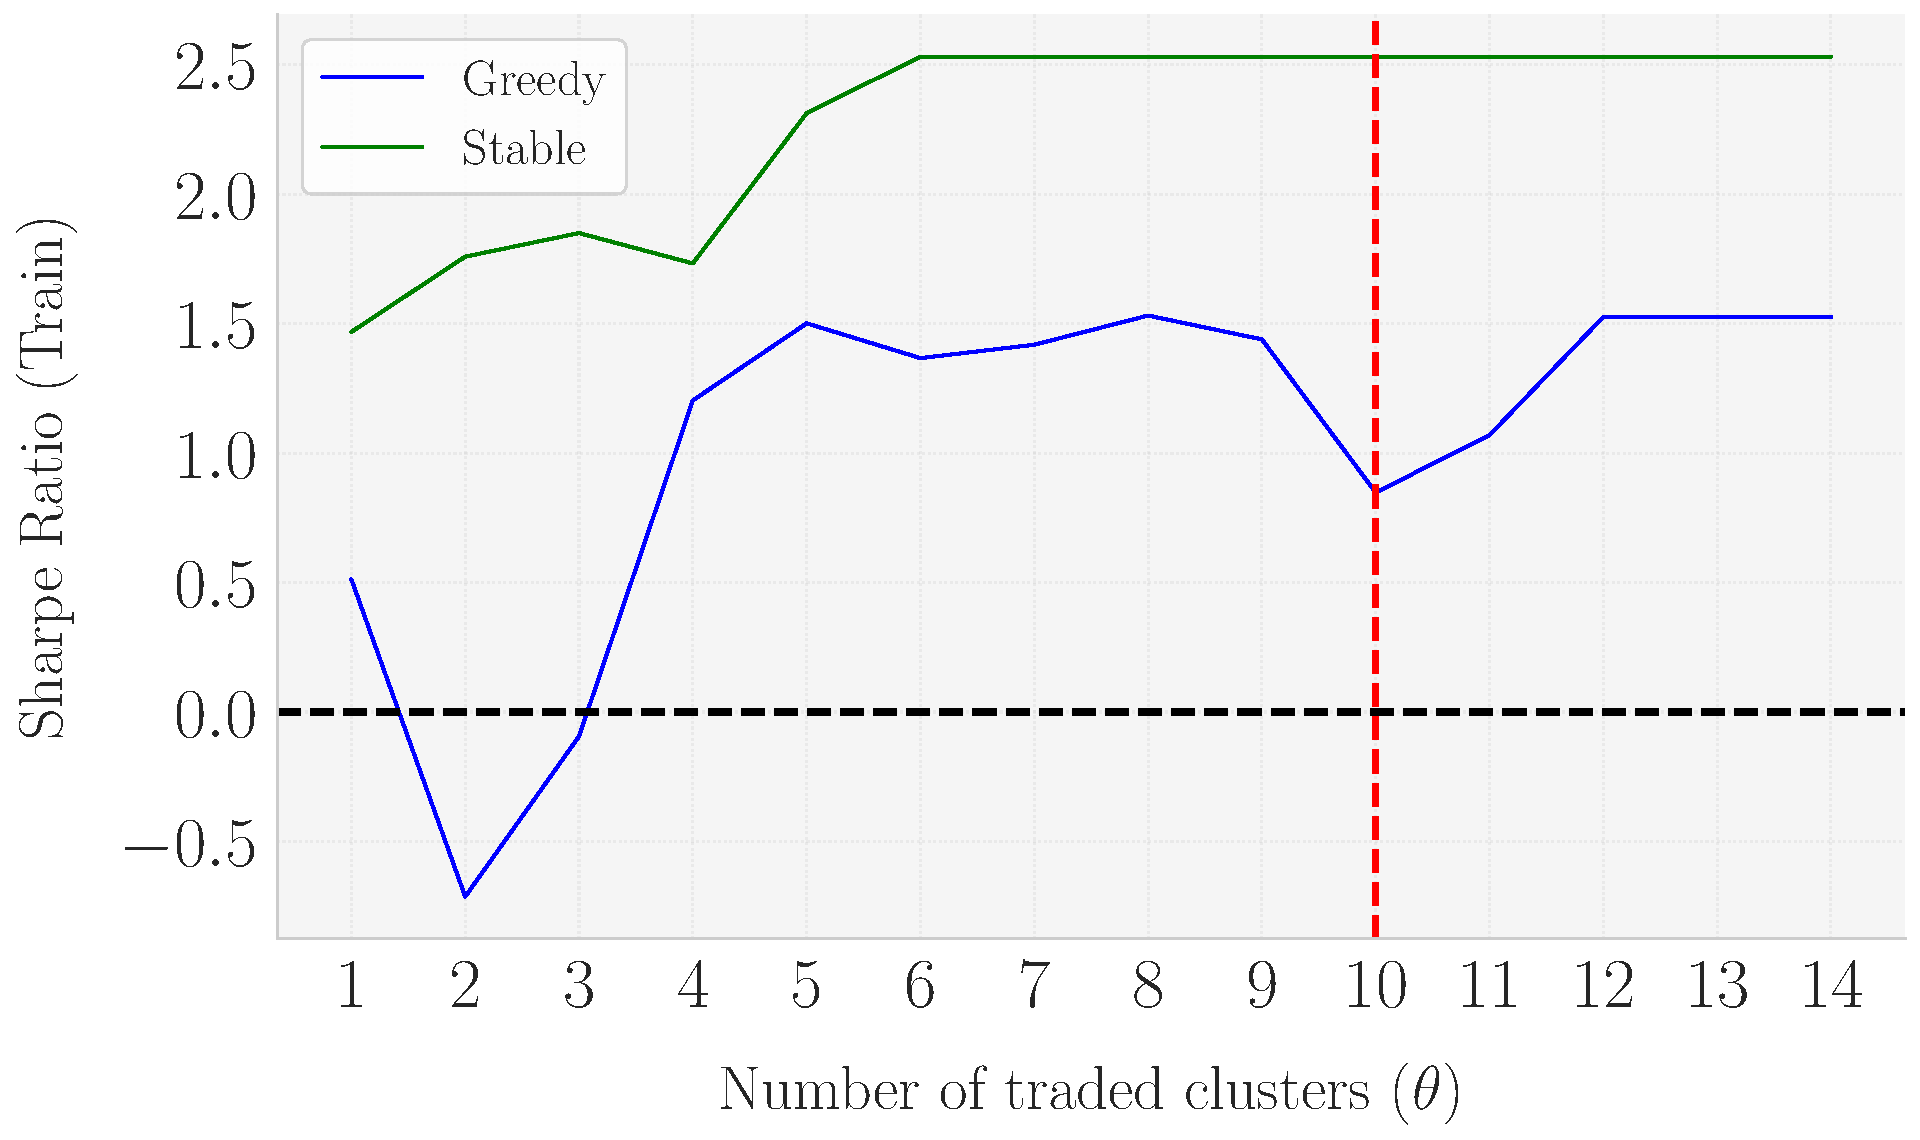
\includegraphics[width=\textwidth]{fig_A4a_LLAMA_SR_Train_vs_theta.pdf}
    \caption{Plot of $SR^{\mathcal P^{tr}}(\theta)$ over a grid of $\theta$}
    \label{fig:LLM_hyp_3}
  \end{subfigure}
  \hspace{0.05\textwidth} % Add horizontal space between the subfigures
  \begin{subfigure}[b]{0.46\textwidth}
    \centering
    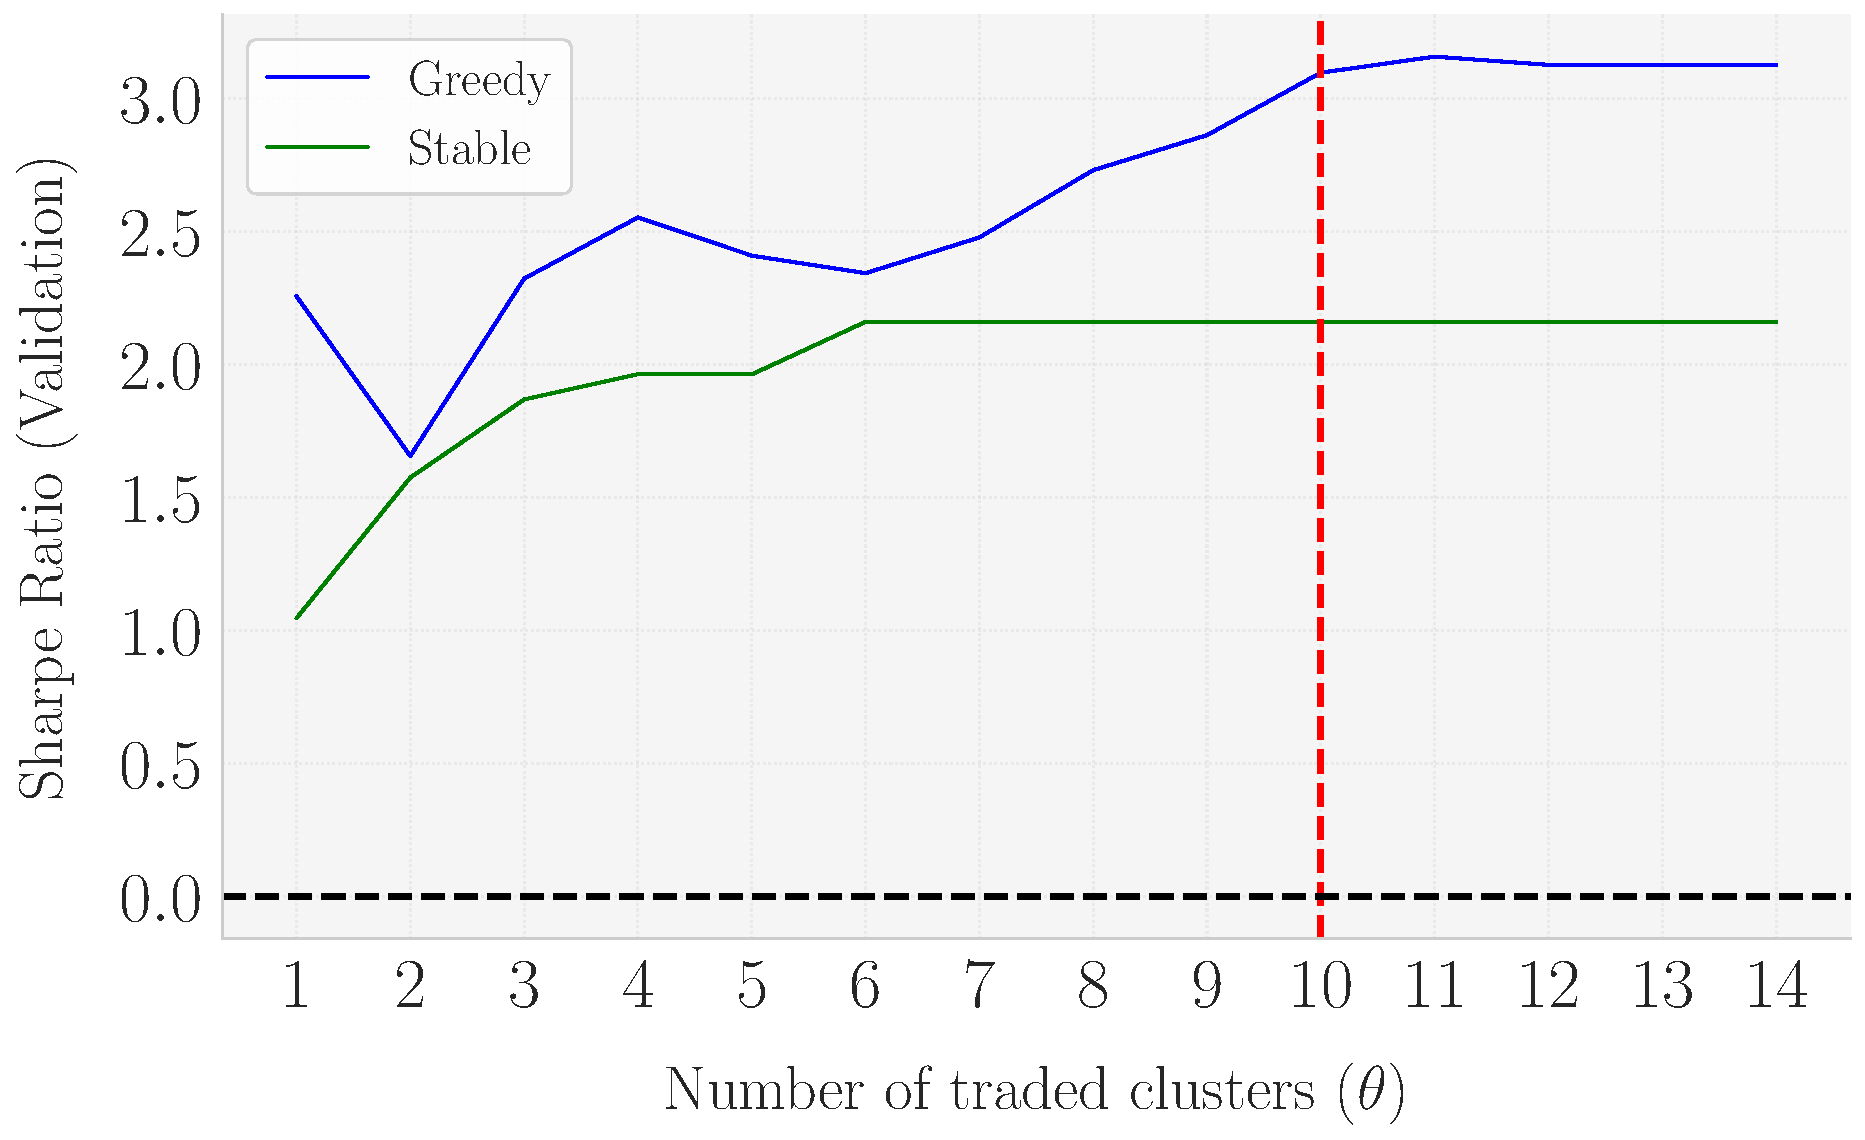
\includegraphics[width=\textwidth]{fig_A4b_LLAMA_SR_Validation_vs_theta.pdf}
    \caption{Plot of $SR^{\mathcal P^{val}}(\theta)$ over a grid of $\theta$}
    \label{fig:LLM_hyp_4}
  \end{subfigure}
\mx
\subcaption*{\textit{Note: This figure illustrates the Sharpe Ratios ($SR$) as a function of $\theta$, the upper bound on the number of traded clusters, for the LLM clustering method in the training (Panel a) and validation (Panel b) splits. In Panel (a), the Sharpe Ratios for the training set indicate a temporary dip at $\theta=10$ for the Greedy algorithm, yet this value still provides a relatively stable outcome. In contrast, Panel (b) shows that $\theta=10$ leads to a noticeable increase in Sharpe Ratios for the validation set, particularly benefiting the Greedy algorithm. The choice of $\theta = \integer{0.5k} = 10$ strikes a balance, confirming it as an effective hyperparameter selection for achieving stability in both the training and validation splits with LLM clustering.}}
\label{fig:LLM_hyperparameter_justification_theta}
\end{figure}
%----------------------------------------------------

